% DESCRIÇÃO DA PROPOSTA--------------------------------------------------------------------

\chapter{DESCRIÇÃO DA PROPOSTA}
\label{chap:descricao}

\section{INTRODUÇÃO}
\label{sec:introducao}
% Introdução-------------------------------------------------------------------------------
O Centro Integrado de Operações da Prefeitura de Belo Horizonte (COP-BH) é a entidade municipal responsável pela integração de informações e da atuação das Instituições envolvidas na resposta a problemas públicos de Belo Horizonte. Suas atividades se baseiam no \textit{Modelo de Gestão Integrada do COP-BH} \cite{ModeloGestaoCOP}, que expressa o seu posicionamento institucional e como promove a integração, alinhamento e harmonização dos processos de trabalho de diversas Instituições e Agências comprometidas com o cuidado da cidade.

Pode ser classificado, segundo a Carta Brasileira para Cidades Inteligentes \cite{CartaCidades}, como um ``Centro de Gestão Integrada - GCI'', sendo este um ambiente estratégico que busca melhorar a eficiência e eficácia da prestação de serviços públicos ao aprimorar a proteção social e governança pública.

O COP-BH viabiliza a integração entre as Instituições e Agências por meio de seis linhas de atuação: \textit{Monitoramento da Cidade, Pronta Resposta, Gestão de Crises, Operações Integradas, Gestão de Eventos e Prevenção de Problemas.}

Conforme o citado modelo \cite{ModeloGestaoCOP}, a linha de atuação de Monitoramento da Cidade possui três vertentes: o monitoramento de sensores não especialistas, tais como câmeras, o monitoramento de sensores especialistas, tais como os meteorológicos, e o monitoramento de fontes de inteligência. Seu objetivo final é permitir que o COP-BH aja preventivamente a fim de evitar problemas públicos ou responder adequadamente a estes, minorando as suas consequências.

Este trabalho analisa e propõe uma mudança no método de análise de dados, bem como sua automatização, para suporte a uma das atividades da linha de atuação de Monitoramento da Cidade, relacionadas ao monitoramento de câmeras, que se delinea a seguir.

\subsection{Contextualização do Projeto}

Conforme descreve o modelo \cite{ModeloGestaoCOP}, a atividade de monitoramento se utiliza de diversos tipos de sensores para sua consecução. Dentre estes sensores, as câmeras instaladas em locais públicos permitem acesso à visualização de diversos pontos da cidade em tempo real.

A atividade de monitoramento das câmeras, ou seja, a visualização das suas imagens em tempo real, é realizada por agentes das Instituições que têm assento no ambiente chamado Sala de Controle Integrado, local onde as imagens são acessadas com o propósito de identificar problemas públicos mais rapidamente, a fim de possibilitar maior celeridade também à resposta.

São diversos os tipos de problemas públicos monitorados, tais como a deposição clandestina de lixo ou inservíveis em locais impróprios, animais de grande porte soltos em via pública, pichação, depredação, acidentes de trânsito, invasão de áreas protegidas e furtos de cabos, entre outros.

Para tornar o serviço mais eficiente, o COP-BH desenvolveu um processo de análise de dados sobre problemas públicos para elaborar um roteiro de monitoramento, que sugere os problemas que devem ser monitorados, os períodos de maior relevância para executar o monitoramento e quais as câmeras deveriam ser monitoradas.

A partir deste roteiro, as equipes de monitoramento teriam um guia de referência que poderia aprimorar o seu trabalho no sentido da eficiência -- pois conheceriam as câmeras deveriam priorizar no monitoramento e quando deveriam ser monitoradas, e da eficácia -- pois isso poderia aumentar a probabilidade de visualizar algum problema público durante o monitoramento.

Para fins deste trabalho, o problema público analisado é o furto de cabos. Para isso, foram utilizados dados reais de ocorrências públicas deste problema em Belo Horizonte, e são originados do Sistema de Gestão de Ocorrências Integradas (SICOP Ocorrências), por meio do qual as Instituições e Agências compartilham informações no COP-BH, Sistema de Gestão da Operação (SGO) utilizado pela BHTrans para controle de suas operações, e dados de furtos de cabos de telefonia compartilhados pelas operadoras de telefonia Oi, Claro, Vivo e V.tal. Estes dados são os mesmos utilizados na elaboração do roteiro de monitoramento. O dataset utilizado para este trabalho contém 18.590 observações sobre o problema de furto de cabos, no período de 03/2018 a 05/2025, e consiste dos seguintes atributos:

\begin{itemize}
  \item{\texttt{origem}, que apresenta de qual sistema os dados se originaram;}
  \item{\texttt{data\_hora}, que apresenta a data e hora em que o furto ocorreu;}
  \item{\texttt{mes\_ano}, que apresenta o mês e ano da ocorrência (dados adicionados para facilitar a análise);}
  \item{\texttt{trimestre\_ano}, que apresenta o trimestre e ano da ocorrência (dados adicionados para facilitar a análise);}
  \item{\texttt{latitude} e \texttt{longitude}, que apresenta a localização exata da ocorrência; e}
  \item{\texttt{endereco} e \texttt{regional}, que apresenta o endereço físico aproximado da ocorrência.}
\end{itemize}

\subsection{Definição do Problema}

Atualmente, o COP-BH elabora o roteiro de monitoramento agrupando as ocorrências pela sua localização, e utiliza o método de estimativa de densidade de kernel para gerar um mapa de calor geoespacial (\textit{heatmap}) \cite{Wilkinson2009} para demonstrar visualmente as regiões da cidade de Belo Horizonte onde há maior concentração de furtos, utilizando a ferramenta de sistema de informação geográfica QGIS \cite{Qgis}. Então, dados de localização das câmeras públicas da cidade são sobrepostos ao mapa de calor, sendo este o resultado final do roteiro de monitoramento, conforme demonstrado na Figura \ref{fig:mapa_roteiro}.

\begin{figure}[!htb]
  \captionsetup{singlelinecheck=false}
  \centering
  \includegraphics[scale=1,keepaspectratio]{dados/images/mapa_roteiro.png}
  \caption{Roteiro de Monitoramento: Mapa de calor de locais de furtos de cabos em Belo Horizonte, com sobreposição de câmeras públicas.}
  \fonte{Produção própria}
  \label{fig:mapa_roteiro}
\end{figure}

Contudo, a análise de dados agregados, na forma como é feita, pode levar a interpretações incorretas. Como se poderá verificar na Figura \ref{fig:grafico_barras_ocorrencias_ano}, que demonstra a evolução dos eventos de furtos de cabo nos últimos anos, houve um aumento abrupto ocorrido do ano de 2022 para o ano de 2023, devido ao acréscimo de dados das operadoras Claro, Vivo e V.tal. Conquanto haja uma aparente e relativa estabilização do ano de 2023 para 2024, não se pode extrapolar projetando a linha de tendência para o ano de 2025. A regressão linear, ao representar apenas a tendência média, é inerentemente limitada para modelar mudanças bruscas de comportamento, como a ocorrida de 2022 para 2023.

Essa limitação é um problema bem documentado na literatura estatística, pois a inclinação do modelo pode ser artificialmente influenciada, mascarando a verdadeira natureza dos dados e novos padrões de comportamento, conforme estabeleceu \cite{Anscombe1973}. Além disso, conforme \cite{Gujarati2011}, ``mudanças estruturais'' nos dados, como a ocorrida no dataset, invalidam a suposição de os parâmetros seriam constantes ao longo do tempo, o que é fundamental para um modelo de regressão único.

\begin{figure}[!htb]
  \captionsetup{singlelinecheck=false}
  \centering
  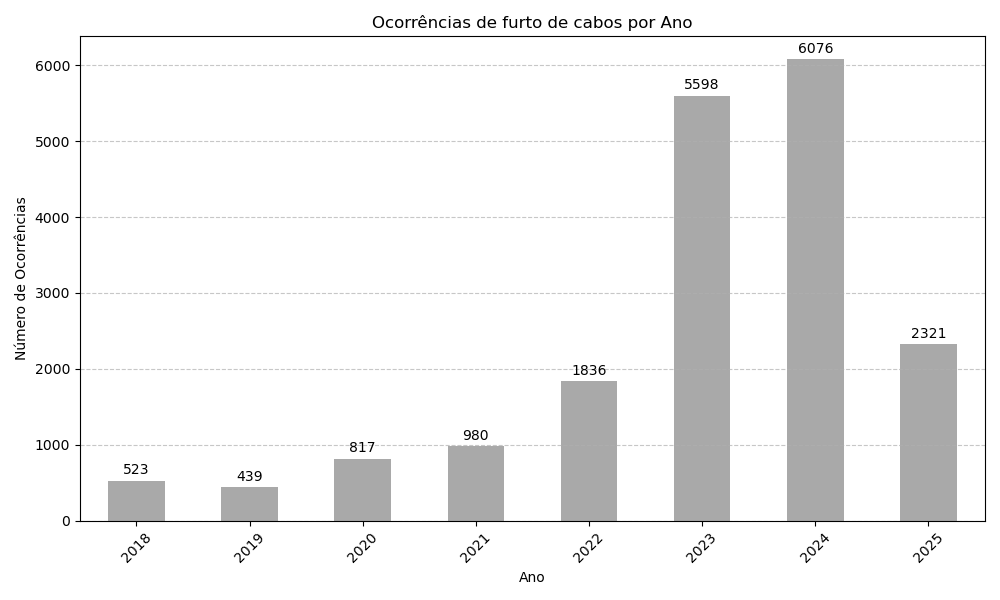
\includegraphics[scale=0.5,keepaspectratio]{dados/images/grafico_barras_ocorrencias_ano.png}
  \caption{Evolução dos eventos de furtos de cabo em Belo Horizonte, no período de 03/2018 a 05/2025.}
  \fonte{Produção própria}
  \label{fig:grafico_barras_ocorrencias_ano}
\end{figure}

Além disso, o simples incremento de novas observações ao conjunto de dados pode ocultar ou impedir a captura de alterações e mudanças, que embora possam parecer sutis, são de fundamental importância para a eficácia da análise, tais como alterações na localização das concentrações do fenômeno e sazonalidades.

Conforme concluiu Robinson \cite{Robinson1950}, erros podem ser cometidos, ou conclusões equivocadas podem ser obtidas ao se inferir comportamentos individuais a partir de estatísticas de dados agregados, a chamada ``falácia ecológica'' (\textit{``Ecological Fallacy''}). Seu estudo estabeleceu formalmente o problema, mostrando como correlações em nível de grupo (estados, cidades, por exemplo) podem ser completamente diferentes ou até opostas às correlações em nível individual.

Por sua vez, Weisburd \cite{Weisburd2015} complementou este entendimento, ao argumentar pela necessidade de ir além da análise de dados agregados, e buscar padrões espaciais por meio de \textit{hotspots}, ou pontos quentes, onde há concentração de crimes.

Acrescenta-se, ainda, o efeito de deslocamento geográfico (\textit{``displacement''}) conceituado por Barr \cite{Barr1990}, que explorou as diferentes formas como o crime se move em resposta a ações de prevenção. As figuras apresentadas na Tabela \ref{tab:tabela_mapas} representam, empiricamente, esse deslocamento espacial dos eventos de furto de cabo em Belo Horizonte, além de indicar as diferentes concentrações dos eventos no tempo. Para fins deste comparativo foram considerados apenas os anos de 2023 e 2024, por serem os anos em que há maior volume de dados no dataset.

\begin{table}[htbp]
  \centering
  \begin{tabular}{|m{3.5cm}|m{3.5cm}|m{3.5cm}|m{3.5cm}|}
    \hline
      \begin{minipage}{\linewidth}
        \centering
        \includegraphics[width=3.5cm]{dados/images/mapa_20231_2.png}
        \captionof{figure}{1T 2023}
      \end{minipage}
      &
      \begin{minipage}{\linewidth}
        \centering
        \includegraphics[width=3.5cm]{dados/images/mapa_20232_2.png}
        \captionof{figure}{2T 2023}
      \end{minipage}
      &
      \begin{minipage}{\linewidth}
        \centering
        \includegraphics[width=3.5cm]{dados/images/mapa_20233_2.png}
        \captionof{figure}{3T 2023}
      \end{minipage}
      &
      \begin{minipage}{\linewidth}
        \centering
        \includegraphics[width=3.5cm]{dados/images/mapa_20234_2.png}
        \captionof{figure}{4T 2023}
      \end{minipage}
    \\ \hline
      \begin{minipage}{\linewidth}
        \centering
        \includegraphics[width=3.5cm]{dados/images/mapa_20241_2.png}
        \captionof{figure}{1T 2024}
      \end{minipage}
      &
      \begin{minipage}{\linewidth}
        \centering
        \includegraphics[width=3.5cm]{dados/images/mapa_20242_2.png}
        \captionof{figure}{2T 2024}
      \end{minipage}
      &
      \begin{minipage}{\linewidth}
        \centering
        \includegraphics[width=3.5cm]{dados/images/mapa_20243_2.png}
        \captionof{figure}{3T 2024}
      \end{minipage}
      &
      \begin{minipage}{\linewidth}
        \centering
        \includegraphics[width=3.5cm]{dados/images/mapa_20244_2.png}
        \captionof{figure}{4T 2024}
      \end{minipage}
    \\ \hline
  \end{tabular}
  \caption{Comparação dos mapas de calor por densidade de kernel das observações de furtos de cabo em Belo Horizonte, dos anos de 2023 e 2024, por Trimestre.}
  \fonte{Produção própria}
  \label{tab:tabela_mapas}
\end{table}

Estes fatos corroboram o entendimento de que o método atualmente utilizado pelo COP-BH ainda é insuficiente para uma análise adequada do fenômeno, além do fato de ser executado manualmente. Assim, esse trabalho busca propor um novo método de análise, bem como uma ferramenta para automatizar este processo.

\subsection{Relevância do Problema}

A atividade de monitoramento é realizada sob a perspectiva da prevenção e pronta resposta à ocorrência de crimes, e nesse contexto o crime de furto de cabos. Esse crime tem diversas consequências negativas, tanto econômicas quanto sociais.

Do ponto de vista social e comunitário, podemos citar diversos problemas que o furto de cabos proporcionam à população em geral, tais como a interrupção de serviços de água, luz, acesso à Internet, serviços de saúde, e transtornos nos sistemas de tráfego e transporte público da cidade  (\citenum{Cemig}, \citenum{OGlobo}, \citenum{R7}, \citenum{OTempoA}, \citenum{OTempoB} e \citenum{HojeEmDia}).

Além disso, há também o impacto econômico, pois o restabelecimento destes serviços demanda o gasto com reparos na infraestrutura de rede elétrica, de telefonia ou de dados, seja pela Administração Pública ou por Concessionárias (\citenum{EstadoDeMinasB}). Pequenos comerciantes e prestadores de serviços também sofrem impactos econômicos decorrentes da interrupção destes serviços essenciais ao funcionamento dos seus estabelecimentos (\citenum{OTempoB}).

Por fim, citam-se os riscos à integridade física dos próprios cometedores deste crime estão expostos, pois podem ser eletrocutados ao manipular cabos e fios de alta tensão, sem as devidas proteções, ou sofrer quedas de altura, ao subir em postes sem equipamentos próprios para isso (\citenum{EstadoDeMinas}).

Portanto, pode-se perceber que o furto de cabos é um problema público importante, causador de diversos transtornos, e que no âmbito do COP-BH é enfrentado por meio do monitoramento por câmeras e correspondente pronta resposta. Neste sentido, ao buscar o aprimoramento da análise de dados em subsídio ao monitoramento inteligente, este trabalho se propõe a contribuir com o enfrentamento ao furto de cabos, que atinge a diversas cidades brasileiras.

\subsection{Justificativa}

O furto de cabos é um problema é reconhecidamente importante e já existem esforços para resolvê-lo. A própria existência de um processo de trabalho no COP-BH que objetiva a elaboração de um roteiro de monitoramento de furtos de cabos já justifica a importância do tema, pois demonstra que a Instituição reconhece o impacto nocivo à cidade, e busca ativamente otimizar a vigilância.

Contudo, a abordagem atual possui lacunas críticas que limitam sua eficácia. A metodologia atual, baseada na agregação de todo o histórico de dados em um único mapa de calor estático, se mostra vulnerável a falácias estatísticas, como a falácia ecológica. Ao tratar dados de anos diferentes com o mesmo peso, o método mascara tendências recentes, sazonalidades e, crucialmente, o deslocamento geográfico do crime. Conforme o dataset utilizado, um hotspot de 2022 pode não ter relevância para o monitoramento hoje, mas continua influenciando o mapa de calor atual, diluindo a importância de novos focos e enviesando a compreensão da movimentação do crime.

Tal como já demonstrado, o furto de cabos não é estático, ele se adapta às ações de repressão e resposta. Assim, esse trabalho se justifica pela necessidade de que a análise dos dados seja, também, dinâmica e adaptativa. É preciso compreender para onde as concentrações de furto estão se movimentando, e quando são mais intensas.

Portanto, é necessário desenvolver e implementar uma solução aprimorada e automatizada, que preencha as lacunas e insuficiências identificadas a fim de se obter melhores resultados.

Com isso, espera-se que, além do aperfeiçoamento na prevenção ao furto de cabos, o modelo metodológico e tecnológico proposto poderá ser adaptado para o combate a outros problemas públicos, fortalecendo a atuação do COP-BH, e contribuindo para uma gestão urbana mais inteligente e segura em Belo Horizonte.

\subsection{Desafios do Projeto}

Pode-se antecipar alguns desafios para o trabalho, sendo que alguns deles poderão ser contornados ou mitigados durante a própria execução. Outros, contudo, somente após a implementação, por meio de acompanhamento por um período de testes. Além disso há aqueles que dependerão de percepções externas do comportamento do fenômeno, por equipes operacionais na ponta. Estes últimos poderão ser melhor tratados em evoluções futuras deste trabalho. Tem-se:

\begin{itemize}
  \item{Padronização dos dados: tendo em vista as variadas fontes dos dados, a automatização deverá levar em conta a normalização dos dados, principalmente quanto ao georreferenciamento;}
  \item{Classificação dos dados: a diversidade de fontes de dados pode ensejar, também, formas e padrões diferentes de classificação;}
  \item{Subnotificação dos dados: pode ocorrer que nem todos os registros de furtos de cabos sejam reportados, ou que sejam reportados com dados imprecisos de data e hora do fato e localização;}
  \item{Disponibilidade dos dados: o dinamismo da análise, com sua automatização, pode ser prejudicado se não houver um meio de capturar os dados de forma rápida;}
  \item{Viéses nos dados: pode ser que os dados estejam sendo capturados em maior volume em locais onde há a presença recorrente de agentes, e em locais onde essa presença seja escassa esteja ocorrendo em igual ou maior volume, mas sem o correspondente registro;}
  \item{Insuficiência de dados: variáveis externas, que também podem ter influência no fenômeno, ainda não estão sendo consideradas;}
  \item{Avaliação da efetividade: pode haver dificuldade em determinar isoladamente se (ou o quanto) o novo método foi eficaz na redução da observação do fenômeno.}
\end{itemize}

\subsection{Contribuição}

Espera-se que este trabalho possa contribuir de múltiplas formas, e em diferentes esferas:

\begin{itemize}
  \item{Com o COP-BH, ao propor um aprimoramento do processo de trabalho de análise de dados e elaboração do roteiro de monitoramento, tornando-o mais dinâmico, preciso e eficiente;}
  \item{No âmbito científico e acadêmico, ao buscar a validação de teorias em contexto real, no que se refere à análise de hotspots e deslocamento geográfico do crime;}
  \item{Por fim, com os munícipes de Belo Horizonte em geral, ao potencializar a capacidade do COP-BH para prevenir o problema público do furto de cabos e suas consequências.}
\end{itemize}

\section{OBJETIVOS}
\label{sec:objetivos}
\subsection{Objetivo Geral}
\label{subsec:objgeral}
%-----------------------------------------------------------------------------------------

% Objetivo Geral--------------------------------------------------------------------------
Este trabalho tem por objetivo geral a melhoria do processo de análise de dados e elaboração do roteiro de monitoramento de furtos de cabos do COP-BH, com o intuito de torná-lo mais preparado a mudanças estruturais nos dados, e aprimorar a precisão no monitoramento, a fim de aumentar a sua eficácia.

Portanto, será desenvolvida e validada uma metodologia computacional automatizada para a análise dinâmica de hotspots de furto de cabos em Belo Horizonte, em suporte às atividades de monitoramento e tomada de decisão tática e operacional do COP-BH.

Cabe salientar que o escopo desse trabalho delimita-se na análise de padrões a partir dos dados que o COP-BH atualmente utiliza, com o mesmo dataset. Portanto não se aprofundará nas dimensões sociológicas, econômicas ou criminológicas que motivam o crime de furto de cabos. O objetivo não é explicar as causas primárias do fenômeno, mas sim a modelar seus padrões de ocorrência no espaço e no tempo de forma precisa e dinâmica.

Dessa forma, a presente pesquisa se caracteriza como um trabalho de ciência de dados aplicada à segurança pública, com ênfase no desenvolvimento e na validação de uma nova abordagem metodológica computacional.
%-----------------------------------------------------------------------------------------

\subsection{Objetivos Específicos}
\label{subsec:objespc}
% Objetivos Específicos-------------------------------------------------------------------
\begin{enumerate}
  \item{Realizar um diagnóstico da metodologia de elaboração do roteiro de monitoramento e do dataset de furtos de cabos atualmente utilizados no COP-BH, para identificar limitações estatísticas e operacionais do processo de trabalho e na caracterização eficiente dos padrões do crime;}
  \item{Desenvolver um modelo computacional para a detectar, de forma dinâmica e automatizada, \textit{hotspots} de furtos de cabo, que combine a análise de tendências temporais, a identificação de mudanças estruturais nos dados e a análise de concentração espacial das observações.}
  \item{Implementar a metodologia desenvolvida em um protótipo capaz de processar as fontes de dados de forma automatizada e gerar, periodicamente, mapas e roteiros que darão suporte ao trabalho das equipes de monitoramento.}
  \item{Avaliar a eficiência do novo método quanto à capacidade de identificar novas áreas de risco, e se adaptar a mudanças estruturais no dataset, bem como ao processo de trabalho de elaboração dos roteiros de monitoramento gerados pela ferramenta com o métido atual.}
\end{enumerate}
%-----------------------------------------------------------------------------------------

\section{TRABALHOS CORRELATOS}
\label{sec:estadoarte}
% Estado da Arte--------------------------------------------------------------------------
A análise criminal é um campo interdisciplinar que envolve ciências de diversas áreas do conhecimento, tais como Criminologia, Geografia, Estatística e, mais recentemente, a Computação. O seu propósito primordial pode ser entendido como a busca por respostas sobre quando, onde e porque o crime ocorreu, evoluindo para quando e onde ocorrerá, seja para prevenir ou reprimir a sua ocorrência.

O trabalho de David Weisburd \cite{Weisburd2015} postulou que o crime não ocorre de forma aleatória no espaço, mas se concentra em locais específicos onde há uma convergência de oportunidades. Formalizou esse entendimento através da ``Lei da Concentração do Crime'', demonstrando que algumas pequenas regiões são responsáveis pela maioria dos eventos criminais em uma cidade.

A partir dessa premissa, o mapeamento criminal passou a adotar técnicas mais sofisticadas, como a Estimativa de Densidade de Kernel (KDE), que é amplamente adotada como um padrão para a visualizar de hotspots -- áreas de alta concentração criminal -- visualmente intuitivos, que facilitam o entendimento da distribuição histórica do crime. Cheiney \cite{Chainey2008} comparou o uso de mapas temáticos por área, elipses espaciais, grades e o KDE, sendo este o que teve melhores resultados para a análise retrospectiva, baseada em dados históricos, estabelecendo-o como um padrão preditivo da ocorrência de crimes.

Contudo, como explorado por Barr e Pease \cite{Barr1990}, o crime se move no tempo e no espaço, e o KDE não tem a capacidade de se adaptar a mudanças bruscas e novas dinâmicas, por sua natureza estática. Portanto, esse trabalho busca uma melhoria dessa ferramenta, procurando incorporar a dinâmica do tempo à análise.

Para capturar a dimensão temporal, e ainda as mudanças estruturais que podem ocorrer nos dados, podemos citar algumas referências principais:

\begin{enumerate}
  \item{Bai e Perron \cite{BaiAndPerron1998} desenvolveram um método de detecção de pontos de mudança (\textit{change point detection}), para análise de séries temporais e mudanças estruturais. A partir deste trabalho, tornou-se possível identificar estatisticamente os momentos em que uma tendência se altera, evitando conclusões equivocadas baseadas em regressões lineares únicas.}
  \item{Kulldorff \cite{Kulldorff1997}, em seu trabalho ``A Spatial Scan Statistic'', estabeleceu o padrão para encontrar \textit{clusters} com significância estatística. Contudo, utiliza formas geométricas simples (círculos e elipses) para escanear o espaço. Isso significa que o hotspot pode não ser bem representado, se tiver uma forma mais complexa ou irregular, ao seguir o traçado de uma via pública, por exemplo.}
  \item{A dimensão temporal foi integrada por Kulldorff et al. \cite{Kulldorff2005} em seu trabalho ``A space-time permutation scan statistic for disease outbreak detection''. O artigo aborda a aplicação da estatística de varredura no domínio espaço-temporal para detectar surtos de doenças em tempo real. O método propõe o conceito de cilindro (não mais as formas geométricas de duas dimensões) como janela de varredura, sendo o tempo a terceira dimensão. Seu objetivo é identificar \textit{clusters} em que o número de observações é maior que o esperado, e então detectar hotspots crônicos, ou surtos -- aumento repentino e localizado de eventos.}
  \item{Han et al. \cite{Han2019} ampliaram o trabalho inicial de Kulldorff \cite{Kulldorff1997}, ao propor o uso do KSS (\textit{Kernel Spatial Scan Statistic}), a partir dos próprios contornos de um mapa KDE como formas candidatas a \textit{clusters}. Para determinar essas regiões de forma irregular, é aplicado um teste da razão de verossimilhança para determinar se a quantidade de crimes observada na região é significativa, em relação à área externa.}
\end{enumerate}

Nesse contexto, o estado da arte é utilizar aprendizado de máquina (\textit{Machine Learning}) não apenas para descrever ou diagnosticar, mas para prever a probabilidade de crimes futuros. São diversas as abordagens existentes, e incluem:

\begin{enumerate}
  \item{Uso de modelos estatísticos avançados que modelam o ``contágio'' de crimes em áreas próximas através da técnica ``Processos pontuais auto-excitáveis'', proposta por Mohler et al. \cite{Mohler2011}.}
  \item{Algoritmos de Machine Learning, tais como os clássicos Random Forest, Support Vector Machine e Regressão Logística, e tendências apontadas para o Deep Learning e arquiteturas híbridas, tais como o CNN-LSTM (Redes Neurais Convolucionais e Redes de Memória de Longo Prazo), conforme revisão realizada por Mandalapu et al. \cite{Mandalapu2023} .}
\end{enumerate}

Contudo, a aplicação de ML neste contexto é acompanhada de um debate crítico intenso. Conforme Mandalapu \cite{Mandalapu2023}, existem desafios recorrentes nessa abordagem, como a esparsidade dos dados (muitas áreas com zero crimes), a dificuldade na interpretação de modelos ``caixa-preta'' de Deep Learning e, crucialmente, a falta de atenção às questões éticas e de viés algorítmico (bias) na maioria dos estudos.

Este trabalho se posiciona na intersecção entre a análise espaço-temporal dinâmica e a aplicação operacional, prática, no COP-BH. O estado da arte revela uma distância significativa entre as práticas comuns ainda baseadas em análises estáticas como o KDE e a fronteira da pesquisa acadêmica, que foca em complexos modelos preditivos de ML. 

Autores como Mandalapu et al. \cite{Mandalapu2023} sugerem que o futuro da pesquisa deve focar na criação de modelos mais explicáveis e justos (\textit{fairness}), na integração de fontes de dados ainda mais variadas (como mobilidade urbana e sociológicas) e no desenvolvimento de sistemas que não apenas preveem, mas também ajudam a entender as causas do crime para subsidiar políticas públicas de prevenção.

Este projeto busca preencher essa lacuna ao não saltar diretamente para a previsão, mas ao focar em um passo anterior, fundamental e de alto impacto: a criação de uma ferramenta de diagnóstico e monitoramento dinâmico. 

Sua contribuição reside no desenvolvimento de uma metodologia automatizada que supera a análise estática tradicional, incorporando princípios de detecção de mudança e análise de clusters espaço-temporais, mas que permanece interpretável, robusta e diretamente aplicável à rotina operacional do COP-BH. Em outras palavras, o trabalho visa a elevar a prática atual a um patamar de análise dinâmica, provendo uma base sólida e confiável sobre a qual futuras iniciativas preditivas poderão ser construídas.
%-----------------------------------------------------------------------------------------

\section{METODOLOGIA DE DESENVOLVIMENTO}
\label{sec:metodologia}
% Procedimentos Metodológicos/Metodologia-------------------------------------------------
Este trabalho tem o objetivo final de propor a evolução da metodologia de análise de dados criminais (mais especificamente, o furto de cabos em Belo Horizonte) atualmente utilizada pelo COP-BH. Neste sentido, pode ser caracterizado como de natureza aplicada, com pesquisa quantitativa e qualitativa. O seu desenvolvimento foi estruturado em quatro fases sequenciais, demonstradas visualmente na Figura \ref{fig:fluxograma_metodologia_final}, e delineadas a seguir:

\begin{figure}[htbp]
    \centering
    \begin{tikzpicture}[
        % Distâncias: 1cm na vertical (dentro dos blocos), 4cm na horizontal (entre os blocos)
        node distance=1cm and 2cm,
        process/.style={
            rectangle, 
            rounded corners, 
            draw, 
            text centered, 
            text width=3.4cm, 
            minimum height=1.2cm,
            font=\footnotesize
        },
        decision/.style={
            diamond, 
            draw, 
            aspect=1.8, 
            text centered, 
            text width=2.8cm,
            font=\footnotesize
        },
        terminator/.style={
            ellipse, 
            draw, 
            fill=gray!20,
            font=\footnotesize
        },
        fitbox/.style={
            draw, 
            rounded corners, 
            inner ysep=0.5cm, 
            inner xsep=0.3cm,
            label={[font=\footnotesize\bfseries]above:#1}
        },
        arrow/.style={
            thick, 
            ->, 
            >=Stealth
        }
    ]

    % --- LINHA SUPERIOR (Fases 1, 2, 3) ---

    % Fase 2 (Centro - Âncora principal)
    \node (D) [process] {Definição da Janela Temporal de Análise};
    \node (E) [process, below=of D] {Aplicação do Método de Detecção de Hotspots};% \\ \tiny\textit{(ex: KSS)}};
    \node (F) [process, below=of E] {Desenvolvimento da Análise de Dinâmica};% \\ \tiny\textit{(Comparação entre janelas)}};

    % Fase 1 (À Esquerda da Fase 2)
    \node (A) [process, left=of D] {Revisão Bibliográfica};
    \node (B) [process, below=of A] {Análise do Processo Atual do COP-BH};
    \node (C) [process, below=of B] {Pré-processamento e AED};

    % Fase 3 (À Direita da Fase 2)
    \node (G) [process, right=of D] {Definição da Arquitetura e Tecnologias};
    \node (H) [process, below=of G] {Codificação da Ferramenta Automatizada};
    \node (I) [process, below=of H] {Geração de Relatórios e Mapas Visuais};


    % --- BLOCOS INFERIORES ---

    % Fase 4 (Abaixo das Fases 2 e 3, com maior espaçamento vertical)
    \node (J) [process, below=of F, node distance=4cm, xshift=3cm, yshift=-2cm] {Definição de Métricas};% \\ \tiny\textit{(ex: PAI)}};
    \node (K) [process, below=of J] {Execução de Testes Comparativos};% \\ \tiny\textit{(Novo vs. Tradicional)}};
    \node (L) [process, below=of K] {Análise dos Resultados};% \\ \tiny\textit{(Quantitativos e Qualitativos)}};

    % Conclusão (Abaixo das Fases 1 e 2, e à esquerda da Fase 4)
    \node (M) [decision, left=of K] {Resultados Satisfatórios?};
    \node (N) [process, below=of M] {Análise Final e Escrita da Dissertação/Tese};
    \node (O) [terminator, below=of N, node distance=1cm] {Fim};
    
    
    % --- AGRUPAMENTO DAS FASES (CAIXAS) ---
    \node [fitbox={1: Diag. e AED}, fit=(A)(B)(C)] {};
    \node [fitbox={2: Modelagem}, fit=(D)(E)(F)] {};
    \node [fitbox={3: Implementação}, fit=(G)(H)(I)] {};
    \node [fitbox={4: Validação}, fit=(J)(K)(L)] {};
    \node [fitbox={Conclusão}, fit=(M)(N)(O)] {};
    
    
    % --- CONEXÕES (SETAS) ---
    % Fluxo interno dos blocos
    \path [arrow] (A) edge (B);
    \path [arrow] (B) edge (C);
    \path [arrow] (D) edge (E);
    \path [arrow] (E) edge (F);
    \path [arrow] (G) edge (H);
    \path [arrow] (H) edge (I);
    \path [arrow] (J) edge (K);
    \path [arrow] (K) edge (L);
    \path [arrow] (M) edge node[right, font=\tiny] {Sim} (N);
    \path [arrow] (N) edge (O);
    
    % Conexões curvadas entre as fases
    \draw [arrow] (C.east) to[out=-30, in=160, looseness=0.8] node[above, sloped] {} (D.west); % Fase 1 -> Fase 2
    \draw [arrow] (F.east) to[out=-30, in=160, looseness=0.8] node[above, sloped] {} (G.west); % Fase 2 -> Fase 3;
    \draw [arrow] (I.south) to[out=-60, in=-340, looseness=1] node[right, sloped] {} (J.east);   % Fase 3 -> Fase 4
    \draw [arrow] (L.west) to[out=60, in=-350, looseness=0.8] node[above, sloped] {} (M.east); % Fase 4 -> Conclusão
    
    % Seta do loop (Não)
    \draw [arrow, dashed] (M.north) to[out=135, in=-90, looseness=0.8] node[above, sloped] {Não} (F.south);

    \end{tikzpicture}
    \caption{Fluxograma da metodologia de pesquisa proposta (Layout Final Ajustado).}
    \label{fig:fluxograma_metodologia_final}
\end{figure}

\subsection{Fase 1: Análise de Dados}

Corresponde ao Objetivo Específico 1, e consiste na compreensão do problema, do processo atual e do dataset.

\begin{enumerate}
  \item{Revisão bibliográfica: Identificação de trabalhos nas áreas de Análise Espaço-Temporal, métodos de criação de \textit{clusters} (KDE, Estatística de Varredura Espacial e Espaço-Temporal) e Detecção de pontos de mudança em dados.}
  \item{Análise do processo atual do COP-BH: Análise qualitativa do processo utilizado no COP-BH, por meio da análise documental dos roteiros de monitoramento existentes e entrevistas não estruturadas com agentes operacionais, para identificação de desafios.} 
  \item{Análise dos dados:}
  \begin{itemize}
    \item{Tratamento dos dados: consolidação, limpeza e tratamento do \textit{dataset}, incluindo a padronização de formatos, tratamento de coordenadas e criação de variáveis agrupáveis.}
    \item{Análise temporal: plotagem da série histórica de ocorrências para identificar tendências, sazonalidades e mudanças.}
    \item{Análise geoespacial: geração de mapas de pontos e de calor com o KDE, para estabelecer a base de comparação com a nova metodologia.}
  \end{itemize}
\end{enumerate}

\subsection{Fase 2: Modelagem e desenvolvimento}

Esta fase corresponde ao Objetivo Específico 2, e refere-se à parte central de revisão da metodologia atual do COP-BH.

\begin{enumerate}
  \item{Definição da unidade temporal de análise: estabelecimento da ``janela de tempo'' para a análise dinâmica. Por ausência de referência inicial, a princípio serão utilizados trimestres conforme demonstrado na Figura \ref{tab:tabela_mapas}, cabendo revisão posterior para uso de outras janelas (bimestrais, semestrais, etc.).}
  \item{Desenvolvimento do modelo de detecção de hotspots:}
  \begin{itemize}
    \item{Será aplicado o método de detecção de \textit{clusters} KSS (\textit{Kernel Spatial Scan Statistic}), analisado por Han et al. \cite{Han2019}, em cada uma das janelas de tempo.}
    \item{Para fins de comparação, a Estatística de Varredura Espaço-Temporal de Kulldorff \cite{Kulldorff2005} também será considerada.}
  \end{itemize}
  \item{Desenvolvimento da análise dinâmica: desenvolver um método para comparar os \textit{hotspots} significativos identificados em janelas de tempo sequenciais (ex.: 1oTri comparado ao 2oTri, e assim sucessivamente). Com isso, pretende-se identificar:}
  \begin{itemize}
    \item{Novos \textit{hotspots}, que não existiam nas janelas de tempo anteriores;}
    \item{\textit{Hotspots} que deixaram de existir, ou se tornaram insignificantes estatisticamente;}
    \item{Mudança na localização dos \textit{hotspots} no espaço;}
    \item{Intensificação ou crescimento de um \textit{hotspot}.}
  \end{itemize}
\end{enumerate}

\subsection{Fase 3: Implementação do protótipo de automatização}

Refere-se ao terceiro Objetivo Específico, e tem por objetivo transformar a metodologia proposta em uma versão inicial de um aplicativo:

\begin{enumerate}
  \item{Definição da arquitetura: pipeline de processamento dos dados e saída dos resultados;}
  \item{Definição das tecnologias utilizadas: a implementação inicial será feita em Python, utilizando bibliotecas padrão do ecossistema de ciência de dados:}
  \begin{itemize}
    \item{Geopandas e Shapely, para manipulação de dados geoespaciais;}
    \item{Scikit-learn, para \textit{clustering} e métricas de avaliação;}
    \item{Pysal, para análise espaciais; e}
    \item{Matplotlib e Seaborn para geração dos mapas e gráficos.}
  \end{itemize}
  \item{Desenvolvimento da automatização do fluxo:}
  \begin{itemize}
    \item{Ingestão contínua de dados;}
    \item{Execução da análise da Fase 2 para a janela de tempo corrente;}
    \item{Geração de relatório visual contendo o mapa de \textit{hotspots} dinâmicos e mudanças detectadas.}
  \end{itemize}
\end{enumerate}

\subsection{Fase 4: Comparação das metodologias}

Refere-se ao quarto Objetivo Específico 4, e objetiva comprovar a eficácia da nova abordagem desenvolvida.

\begin{enumerate}
  \item{Definiçãoda métrica de avaliação: será utilizada a métrica padrão Índice de Acurácia Preditiva (\textit{Predictive Accuracy Index - PAI}) para avaliar os \textit{hotspots} identificados. O PAI é utilizado para medir a eficiência de um mapa de \textit{hotspots} em prever a localização de eventos futuros, conforme o trabalho de Chainey et al. \cite{Chainey2008}: \ref{eq:pai}.\\  }
  \begin{equation} \label{eq:pai}
    \begin{array}{rcl}
      PAI = \frac{Ph}{Qh} \\ \\
      \text{Onde } Ph \text{ é o \% de crimes que ocorrem dentro do \textit{hotspot}} \\
      Qh \text{ é o \% da área total que é coberta pelo \textit{hotspot}} \\
    \end{array}
  \end{equation}
  \item{Análise e comparação visual: serão gerados dois roteiros, A e B, sendo o roteiro A pelo método atual do COP-BH e o roteiro B pelo novo método desenvolvido:}
  \begin{itemize}
    \item{Roteiro A com o mapa de calor com KDE de todos os dados históricos até T1;}
    \item{Roteiro B com o mapa de \textit{hotspots} gerado pela nova metodologia usando apenas os dados de T1;}
    \item{Os dois roteiros serão comparados a um mapa que mostra os dados do trimestre seguinte (T2), para calcular e comparar os índices PAI.}
  \end{itemize}
\end{enumerate}
%-----------------------------------------------------------------------------------------

\section{CONSIDERAÇÕES FINAIS} % Escolher o nome mais adequado ao trabalho
\label{sec:conclusao}
% Conclusão/Considerações Finais----------------------------------------------------------
Este trabalho se propõe a  analisar um fenômeno criminal dinâmico, como o furto de cabos, superando as limitações de uma abordagem estática. Busca implementar uma metodologia computacional automatizada capaz de identificar hotspots de forma dinâmica, analisando o surgimento, o deslocamento e a dissipação de áreas de risco ao longo do tempo. Além disso, utiliza uma avaliação retrospectiva utilizando uma métrica de desempenho reconhecida academicamente, o Índice de Acurácia Preditiva (PAI), ensejando assim, uma evolução no processo de trabalho do COP-BH, do qual já foram identificadas as insuficiências.

Ressalta-se que a validação realizada neste trabalho concentrou-se na eficácia metodológica em um ambiente controlado. Como desdobramento e evolução deste projeto, idealiza-se a realização de uma validação operacional, numa próxima etapa. Dessa forma, a validação operacional consistirá na implementação da ferramenta como um projeto-piloto na rotina do COP-BH, envolvendo o treinamento de agentes de monitoramento e a coleta de dados empíricos sobre seu impacto real na detecção de ocorrências, bem como a análise qualitativa da percepção e da utilidade da ferramenta junto aos agentes operacionais.

Adicionalmente, pretende-se agregar mais dados à análise, e com isso se espera aprimorar significativamente a robustez do modelo. Futuramente, pretende-se enriquecer a análise com dados sociológicos, como o mapeamento de áreas de permanência de moradores em situação de rua, e dados econômicos cruciais. Isso inclui a geolocalização de ferros-velhos e outros potenciais receptadores de cabos furtados, que modelam a cadeia de escoamento do delito, e a incorporação da série histórica da cotação do preço do cobre no mercado internacional, que funciona como um indicador macro do incentivo econômico para este tipo de crime.

Por fim, talvez a aplicação futura mais interessante desta metodologia seja a sua integração com os sistemas gerenciamento de vídeo (\textit{Video Management System} - VMS) que o COP-BH utiliza para o monitoramento. A ideia é utilizar os resultados da análise e identificação de um hotspot emergente para ativar a execução automatizada de analíticos de vídeo específicos nas câmeras que cobrem a área de risco e somente durante a janela de tempo de maior probabilidade. São diversos os problemas públicos monitorados desta forma, para além do furto de cabos, tais como animais soltos em via pública, deposição clandestina de lixo, pixação, depredação, entre outros, que poderiam ser ativados de forma seletiva, provendo inteligência à atividade de monitoramento. A ocorrência de um evento detectado pelo analítico geraria, então, alertas operacionais prioritários para que ações de prevenção ou mitigação, como o empenho de um recurso operacional, pudessem ser tomadas no menor tempo possível.

Em suma, este trabalho busca uma evolução da solução metodológica atual em resposta a um problema operacional conhecido, que pode alicerçar evoluções futuras. A partir dele, espera-se prover proatividade e inteligência, baseadas em evidências, ao trabalho do COP-BH, em sua missão de cuidar da cidade de Belo Horizonte.
%-----------------------------------------------------------------------------------------